\documentclass[oneside]{book}
\setlength\parindent{24pt}
\usepackage{indentfirst}
\usepackage{lmodern}
\usepackage{color}
\usepackage{listings}
\usepackage{graphicx}
\lstset{ %
language=C++,                % choose the language of the code
basicstyle=\footnotesize,       % the size of the fonts that are used for the code
numbers=left,                   % where to put the line-numbers
numberstyle=\footnotesize,      % the size of the fonts that are used for the line-numbers
stepnumber=1,                   % the step between two line-numbers. If it is 1 each line will be numbered
numbersep=5pt,                  % how far the line-numbers are from the code
backgroundcolor=\color{white},  % choose the background color. You must add \usepackage{color}
showspaces=false,               % show spaces adding particular underscores
showstringspaces=false,         % underline spaces within strings
showtabs=false,                 % show tabs within strings adding particular underscores
frame=single,           % adds a frame around the code
tabsize=2,          % sets default tabsize to 2 spaces
captionpos=b,           % sets the caption-position to bottom
breaklines=true,        % sets automatic line breaking
breakatwhitespace=false,    % sets if automatic breaks should only happen at whitespace
escapeinside={\%*}{*)}          % if you want to add a comment within your code
}
\begin{document}
\title{Unofficial Guide to Interning at Wikia}
\author{...well, at least on the Services Team}
\date{July 2015}
\maketitle
\tableofcontents
\chapter{What is this?}
When you join a new team, you have to tackle a huge repository of existing code and a ton of new tools. On top of that, the team will likely have established guidelines for how new code should be written, protocols for the process of committing new code, and a bunch of other unique development practices.\par
The purpose of this guide is to break down the moving parts of the Wikia Services Team into easy-to-understand components. Between IDE's and Mocking Frameworks and Scrum, there will likely be concepts that you are familiar with, as well as concepts that you've never heard of.\par
This guide is meant to be a living document. As time passes, especially in the tech world, tools change. Feel free to update this document as it becomes outdated and new developments occur.
\chapter{How to get started coding}
\section{IntelliJ}
\subsection{Setting up IntelliJ}
The Services Team uses IntelliJ as their Java IDE. The Pandora repository wiki (github.com/Wikia/pandora/wiki/Getting-Started) includes a step-by-step guide on setting up Java and IntelliJ on your machine.
\subsection{I've never used an IDE. What is this and why can't I just use a text editor?}
If used properly, an IDE can save you a ton of time. 
How, you ask?
\begin{itemize}
	\item \textbf{Code Navigation:} \texttt{Command + click} on a function or variable
	\item \textbf{Code Completion:} IntelliJ auto-completes classes and method names as you code. It also expands acronyms (i.e. NPE for "NullPointerException" or "No Page Error."
	\item \textbf{Code Generation:} \texttt{Ctrl + return} can generate getters and setters or implement methods from an interface.
	\item \textbf{Code Coloring:} IntelliJ includes the standard keyword, string, and variable coloring. It also colors member variables, local variables, and parameters.
	\item \textbf{Refactoring:} IntelliJ is extremely effective for mistake-free renaming, even replacing setters, getters, and string usages,
	\item \textbf{Dependency improrting:} When relying on a third party library that you have the source for, you can navigate to the code easily for reference.
	\item \textbf{Debugging:} IntelliJ has a built-in debugger, which we will discuss in-depth in the debugging chapter.
\end{itemize}
\section{What is Pandora?}
The Pandora repository, located at \texttt{github.com/Wikia/pandora}, is where all of Wikia's services are located. All of our Java API's are located in this repo. Pandora also includes all of the tools and support libraries that are central to these services as well as all the tests for these services. As stated on repo's wiki, the purpose of Pandora is to:
\begin{itemize}
	\item Provide a simplified guidelines compliant content interface to articles
	\item Enable rapid prototyping and iteration of the above
	\item Hide the complexity of MediaWiki
	\item Decouple content which will enable HyperMedia API designs, better caching, and the ability to fan-out requests.
\end{itemize}
\section{What is Helios?}
The Helios repository, located at \texttt{github.com/Wikia/helios}, is the authentication service for MediaWiki. It is written in Go. We've decided to treat authentication as user creation instead of just registration.
\subsection{What is Go?}
Go is a static-typed language with syntax that is loosely similar to X. Go emphasizes good composition while delivering “concurrency with the static execution speed of C.” Go supports garbage collection, type safety, dynamic-typing, among other features. 
\section{What is MediaWiki?}
MediaWiki is a large open-source project that was started in 2004.It is written in PHP and provides a lot of core functionality for content management. Wikipedia and Wikia run on MediaWiki. 
\subsection{What big is it?}
MedaWiki is 5 million lines of code, which is part of the reason that it is sometimes extremely difficult to dive right into. These 5 million lines are:
\begin{itemize}
	\item 1/3 core MediaWiki
	\item 1/3 core extensions
	\item 1/3 Wikia extensions
\end{itemize}
\subsection{How does it relate to us?}
As a company, we have decided to slowly move off of MediaWiki and onto our own independent services. Currently, several other teams do a lot of development in MediaWiki, but the services team does not. Our company's long-term goal is to eventually stop creating extensions for MediaWiki and only create services independent of MediaWiki. That is what the services team is working on.
\chapter{Stand-up? Backlog grooming? Demo's? What are all these meetings!}
As you likely noticed from your calendar, the Services Team has a lot of meetings. This is because we use the Agile Process. The Agile Process is a group of software development methodologies that are meant to make our collaboration and self-organization as effective as possible.
\section{What is Scrum?}
Scrum is a subset of Agile. It is a particular set of practices that must be followed for a process to be consistent with the Agile framework. Scrum emphasizes maximizing the amount of productive time available for useful work to get done. 
\section{What are Sprints?}
Sprints are the amount of work to do in a set amount of time. For the Services Team, every sprint starts on a Friday and lasts two weeks.  Before the start of a new sprint, we have \textbf{Backlog Grooming} meeting, where we discuss the tasks that are currently in the backlog and comment on how we will tackle them. Then, we have a \textbf{Sprint Planning} meeting where we choose the number of tasks that we want to get done in the upcoming sprint. At the end of that sprint, we have a \textbf{Demo}, which is a slide presentation that shows off the work that is done. Then, we have a \textbf{Retrospective} meeting, where we look back on the sprint and consider what went well, what didn't go well, and what we will change next sprint. The Retrospective is very important to Scrum because it allows the team to quickly recognize what went wrong and fix it. If a task didn't go as planned or there is a problem with our approach, we can quickly pivot towards a new set of tasks and focus.
\section{What are Stories?}
Stories is a term for an overarching task that needs to get done. Stories only describe \textit{what} needs to get done, not \textit{implementation}. Stories get broken down into \textbf{tickets}, which are smaller components of the larger task. 
\section{What is JIRA?}
Jira is the Project Management Software we use to keep track of our Sprints. You can use it to view our sprint progress, look at our stories and tickets, and create new stories and tickets at \texttt{https://wikia-inc.atlassian.net/}. 
\section{What are problem designations?}
When a problem is discovered, it is given an urgency designation:
\begin{itemize}
	\item P1: This is an \textbf{URGENT} problem. The site is down! Drop everything and fix this immediately.
	\item P2: Something major is broken; fix this within 48 hours.
	\item P3: Something is broken, fix this within 2 weeks.
	\item P4: Everything else goes here!
\end{itemize}
\section{What are Stand-Ups?}
Stand-Ups are daily meeting that we have to discuss the following:
\begin{itemize}
	\item What did I accomplish yesterday?
	\item What will I do today?
	\item What obstacles are impeding my progress?
\end{itemize}
We call them "Stand-Ups" because the members are typically standing. The discomfort of standing is intended to keep these daily meetings concise.
\subsection{Why do they sometimes happen at 8AM?}
Since Wikia has an office in Poznan, some of the Services Team members are in Poland. In order to maintain communication, two Stand-Up meetings a week are held at 8AM via BlueJeans (our video-conferencing platform) between the US and Poland team.
\section{What are the roles?}
There are three main roles in the Scrum process. Team members, Product Owner, and Scrum Master. As of July 2015, Geoff Benson is both the Product Owner and the Scrum Master. The rest of the services team are team members.
\subsection{What do team members do?}
Team members are the majority of the Services Team. They can do whatever they want to get stories done and have flexibility in their approach.
\subsection{What does the Product Owner do?}
The Product Owner is the one who decides what order things need to get done in. He can make overarching decisions regarding the sprint. 
\subsection{What is the Scrum Master?}
The Scrum Master helps make sure the process runs smoothly. The Scrum Master serves as an adviser on the best way to tackle problems and makes recommendations based on past experience. 

\chapter{So many tools! How do I keep track?}
Don't worry! Here is a brief overview of the coding tools that the Services Team uses:
\section{What is Dropwizard?}
The Services Team uses a collection of different libraries in our web services. Dropwizard brings all these libraries together and does the wiring for our \textbf{RESTful services}.
\subsection{What is REST?}
REST stands for Representational State Transfer, and it is a simple way to organize interactions between independent systems. REST is an architecture style for designing networked applications. RESTful applications use HTTP requests to post data (create and/or update), read data (e.g., make queries), and delete data. Thus, REST uses HTTP for all four CRUD (Create/Read/Update/Delete) operations.
\subsection{What is HTTP?}
HTTP is the protocol, or set of rules, that allows for sending documents back and forth on the web. This protocol determines which messages can be exchanges and which messages are appropriate replies to others. \par
In HTTP, there are two different roles: \textbf{server} and \textbf{client}. The client always initiates the conversation and the server replies. HTTP messages are made of a header and a body?
\subsubsection{What is a HTTP message body?}
The body of an HTTP message contains the data you want to transmit over the network. 
\subsubsection{What is a HTTP message header?}
The header of an HTTP message contains metadata, including instructions on how to use the data in the body. In the case of a request, it contains important HTTP methods.
\subsubsection{What is a URI?}
URIs, or Uniform Resource Identifirs, are how you identify the things that you want to operate on. For example, a web page is a type of resource and all webpages can be accessed using a specific type of URI called an URL.
\subsubsection{What are HTTP verbs?}
Each HTTP request specifies a certain HTTP verb, or method, in the request header. This is the first all caps word in the request header. For example, \par
\texttt{GET HTTP/myresource} means the \texttt{GET} method is being used.\par
There are four HTTP verbs: \texttt{GET, PUT, DELETE, POST}. HTTP verbs tell the server what to do with the data identifid by the URI.
\subsubsection{GET} is the simplest type of HTTP request method; browsers use this method each time you click a link or type a URL into the address bar. It instructs the server to transmit the data identified by the URL to the client. Data should never be modified on the server side as a result of a \texttt{GET} request.
\subsubsection{PUT} requests are used when you wish to create a resource identified by a URL. For example,\par
\texttt{PUT /client/connie} \par
might create a client, \texttt{connie}, on the server. 
\subsubsection{DELETE}  
\texttt{DELETE} requests are used to delete the resource identified by the URL of the request. For example, if the user did something undesirable and needed to be removed from the system, we could:
\texttt{DELETE /client/connie}
\subsubsection{POST}  
\texttt{POST} requests are used to update a resource identified by the URL. Unlike all the other HTTP methods, \texttt{POST} requests are not necessarily idempotent.
\texttt{DELETE /client/connie}
\section{Gradle}
Gradle is an extensive build tool and dependency manager for programming projects. Gradle also provides build-by-convention support for many types of projects including Java, Android and Scala.
\subsection{What is a build script?}
Your build scripts are how you tell Gradle how to build your application. The application itself can be represented by many Gradle projects. A Gradle project does not represent your application as a whole, but instead can represent many different things. It could represent a library jar file you want to build for your project, it could be a distribution zip file, or it could just represent something you want done with the app, such as deploying it to a server.\par
One benefit of having multiple projects in a single application is that it simple to have separate dependencies or to build tasks for the different application parts.\par
How does Gradle know what counts as a project in your application? It will create a project for each 'build.gradle' file in your application. On the previous example, both the Mobile and Wear directories in a Wear application would have a 'build.gradle' file letting Gradle know that it is a separate project. For each project in your build, Gradle will create a Project object. This object allows you to access Gradle features such as adding tasks, properties and dependencies. Properties are defined in the 'build.gradle' file, typically in an extra block.
\section{Jrebel}
JRebel instantly reloads changes to Java code and saves developers time. It works as a java agent on top of the JVM. It looks for changes in the folder with your compiled classes. If you compile a class, JRebel notices the change and compares the differences between class definitions. Then at the bytecode level it adds/removes/replaces fields/method bodies/etc. without restarting the JVM.\par
The JRebel Activation Code can be provided by Nelson.
\section{Project Lombok}
Lombok is a tool that generates code for you, but not in the way that your IDE generates it. Your IDE generates getters and setters, or equals and more, and then puts the code in your uncompiled class file. Lombok generates the same thing, but does it in the class file; all you need to do is add some annotations like \texttt{@Setter}, \texttt{@Getter}, \texttt{@Builder}, \texttt{@Data}, etc. to your code and Lombok generates the setters, getters and so on for you. At the same time, you can override whatever is generated by just writing the method yourself instead.\par
Below is an example of using lombok to generate getters and setters using the \texttt{@Data} annotation. \texttt{@Builder} creates a builder for this class, while \texttt{@AllArgsConstructor} and \texttt{@NoArgsConstructor} create constructors:\par
\begin{figure}[h!]
\centering
	\includegraphics[scale=0.5]{lombok.png}
\end{figure}
\section{Guice}
Guide is a dependency injector, or a way to inject objects into your application without having to explicitly reference those objects. For example:
\begin{lstlisting}
@Inject
	public class MyClass(InjectObject injectedobject){
		this.injectedobject = inject object;	
	}
\end{lstlisting}

The above code would provide an instance of InjectedObject into my code, as long as I had the following code in my module (module is Google Guice's term for where you create your bindings and define your dependencies):
\begin{lstlisting}
@Provides
	InjectObject provideInjectObject(){
		InjectObject standardInjectObject = new InjectObject(standardParameters);
		return standardInjectObject;
	}
\end{lstlisting}
\section{Guava}
Guava is a collection of several of Google's core libraries used for Java-based projects. It includes libraries for collections, caching, common annotations, string processing, I/O, and more. We often use Guava in our Java repo, Pandora.
\section{Swagger}
Swagger is a framework for defining your API. For our Java code, we can use Swagger annotations throughout our code. Swagger uses these annotations to automatically create JSON definitions.These definitions can be used to generate documentation as well as generate code.
\chapter{What is Git and why do we use it?}
\section{What is Git?}
Git is a version control system, or VCS. Specifically, it is a distributed VCS.
\section{Why version control?}
Nobody likes to lose their work. Maybe you're the type of person who constantly pounds the "Save" button on your documents or stores all his files in the cloud. VCS address that paranoia. It helps you track changes to your code.\par
Version Control Systems provide a documented history. As you make changes to your code, you will eventually reach a good stopping point. To save the current status of your project, you still mark the files you changed and "commit" your changes to the VCS. The VCS will store exactly how your code looked at that moment. If you make more changes later, but look back and decide that your new changes are bad, you can always restore your code to a previous commit.\par
Version Control Systems also allow teams to work together, all using the same files. If you've ever tried to edit a document with multiple people (without using Google Drive), you've likely run into issues where somebody edits an older version and is stuck adding their changes to the current version. Or worse, they send out their version and overwrite all the new changes. Using git, there is one remote repository that everyone on our team can work on, make locally make changes to, commit their changes to, and pull changes from when the repository is updated.
\section{What is a repository?}
A repository, or "repo", is a directory where your projects can live. Wikia/pandora is a remote repository on Github. You will also have a local repository on your computer. 
\section{What is my local repository?}
Your local repository is a copy of all the files in the remote repository on your own machine. Your local repository
\subsection{I want to start coding! How do I set up my local repository?}
\noindent Download git for OS X (https://git-scm.com/downloads)\par
\noindent Create your working copy of Wikia/pandora:\par
1. Navigate to the folder on your machine where you want to store your local repo.\par
2. Use the terminal for the following command: git clone https://github.com/Wikia/pandora.git \par
\noindent You have a working copy of the entire pandora repository!
\subsection{I got my first ticket! What do I do?}
\noindent Make a branch with your ticket name.\par
This command creates a local copy of all the files in master.\par
\texttt{>>> git branch SERVICES-000} \par
\noindent This command allows you to start working on your branch.\par
\texttt{>>> git checkout SERVICES-000} \par
\noindent Now, you can start making your changes on this branch!
\newpage
\subsection{I just finished coding! What do I do?}
Once your changes are finalized on your branch, push your changes are navigate to the github website to make a pull request. Once you've made your pull request, Jenkins will run unit and integration tests to confirm that your code has not broken anything. This may take a few minutes. If these checks don't all pass, you will need to fix your code. See "What is Jenkins" for more information. \\
\newline
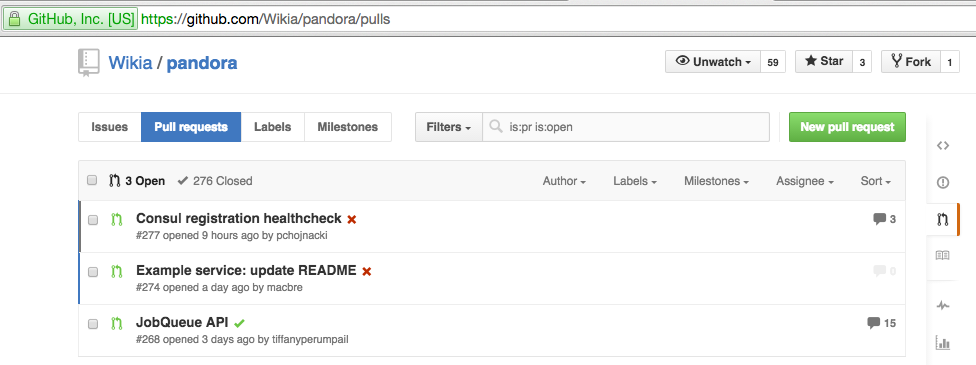
\includegraphics[scale=0.4]{pullrequest.png}
\chapter{What is TunnelBlick?}
Tunnelblick is a free, open source graphic user interface for OpenVPN on OS X. It provides easy control of OpenVPN client and/or server connections.
\subsection{What is a VPN?}
A VPN or Virtual Private Network is a network connection that enables you to create a secure connection over the internet to private networks.\par
Our VPN provides employees with secure remote access to our company network. By connecting to the company's network, an individual employee can access all the company's resources and services on-site as well as remotely.
\begin{figure}[h!]
\centering
	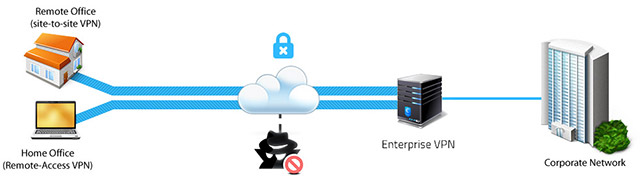
\includegraphics[scale=0.3]{VPN.png}
	\caption{VPN connecting to a Corporate Network}
\end{figure}
\section{What is Jenkins?}
Jenkins is a continuous integration tool written in Java. Whenever you push to the Pandora repo, Jenkins will run all the unit and integration tests as well as health check tests to make sure that the new changes have not broken anything. If your Jenkins tests don't pass, here is what to do: \\
\begin{itemize}
	\item Click details on the failed test:\\
	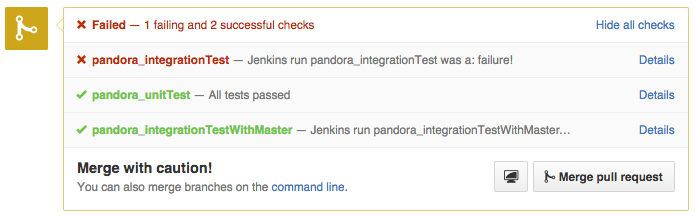
\includegraphics[scale=0.4]{githubtestsfailed.png} 
	\item Navigate to \texttt{Console Output} on the right hand bar:\\
	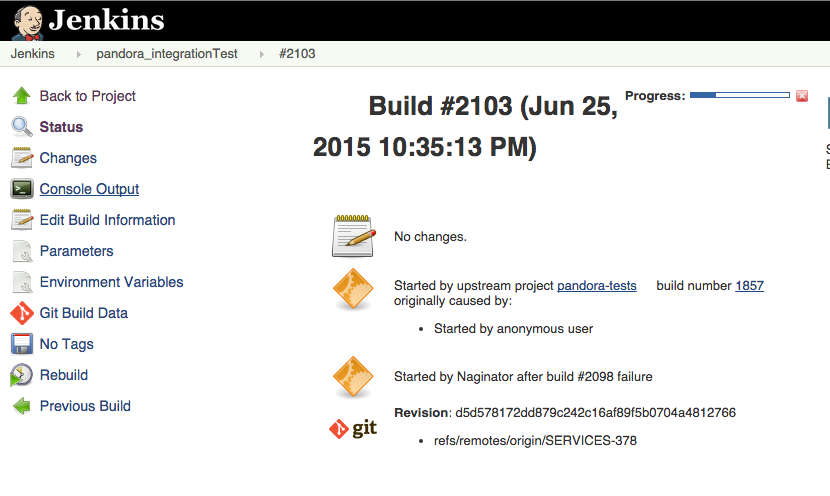
\includegraphics[scale=0.4]{jenkinshome.png}
	\item Scroll down until you find \texttt{BUILD FAILED} in bright red to locate where the error occurred:\\			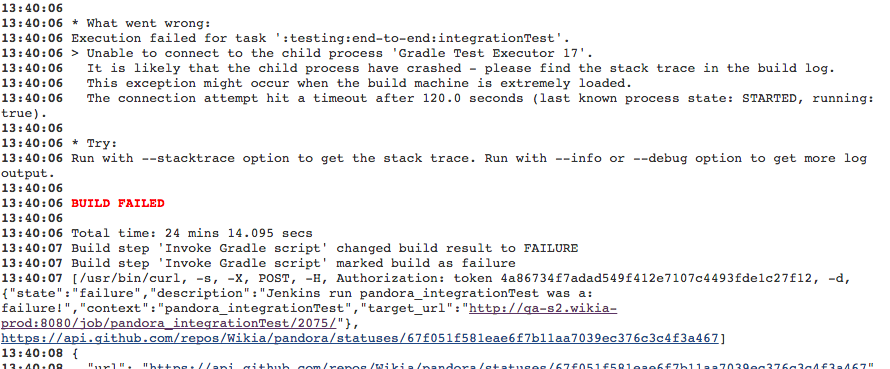
\includegraphics[scale=0.4]{jenkinsbuildfailed.png}
\end{itemize}
\section{What is Vignette?}
Vignette is a thumbnailer. It's a proxy to imagemagick, which you can read more about at \texttt{http://www.imagemagick.org/script/index.php}.
\chapter{How do I debug?}
The first three things I double-check when my code isn't working in the office are:
\begin{itemize}
	\item Am I connected to VPN?
	\item Have I configured my environment variables and argument?
	\item Have I synced Gradle?
\end{itemize}
If none of these checks reveal the problem, then we'll have to delve into using the IntelliJ Debugger.
\section{IDE Debugging}
\subsection{Why use an IDE debugger?}
You may be thinking, why do I need a debugger? I can already look at trace messages in my code. What more do I need!\par
Here are some benefits of using an IDE debugger:
\begin{itemize}
	\item Add \textbf{breakpoints} to temporarily suspend execution of your program at a certain point (No more print-statement debugging!)
	\item Be able to  \textbf{watch variables} and see when they change
	\item Conditional breakpoints; stop the application only in exceptional circumstances to allow you to analyse the stack and variables.
	\item View the call stack at any point in time, giving you a context for your current stack frame.
	\item Change variable values while the program is running
	\item Be able to skip or repeat sections of code, to see how the code will perform. This allows you to test out theoretical changes before making them.
	\item Alert you when certain exceptions are thrown, even if they are handled by the application.
\end{itemize}
\subsection{What are breakpoints?}
A breakpoint is a signal that tells the debugger to temporarily suspend execution of your program at a certain point. When execution is suspended at a breakpoint, your program is said to be in break mode. Entering break mode does not terminate or end the execution of your program. Execution can be resumed at any time.\par
You can think of break mode as being like a timeout. All the elements remain, functions, variables, and objects remain in memory, for example, but their movements and activities are suspended. During break mode, you can examine their positions and states to look for violations or bugs. You can make adjustments to the program while in break mode. You can change the value of a variable, for example. You can move the execution point, which changes the statement that will be executed next when execution resumes.\par
Breakpoints are a powerful tool for pinpointing where a problem is occurring in your code. Rather than stepping through your code line-by-line or instruction-by-instruction, you can allow your program to run until it hits a breakpoint, then start to debug. This speeds up the debugging process enormously. Without this ability, it would be virtually impossible to debug a large program.\newpage
\subsection{How do I do all this in IntelliJ?}
Below is an example screenshot of using the debugger in IntelliJ. By clicking on the gray section to the left of your code, you can add break points, which are represented by red circles (see below). In order to run your code in debug mode, click the green "bug" icon next to the standard run icon. Then, once you hit a breakpoint, you can navigate to the variable tabs on the lower portion of your window to view the current state of the variables. \newline
\newline\begin{flushright}

\end{flushright}
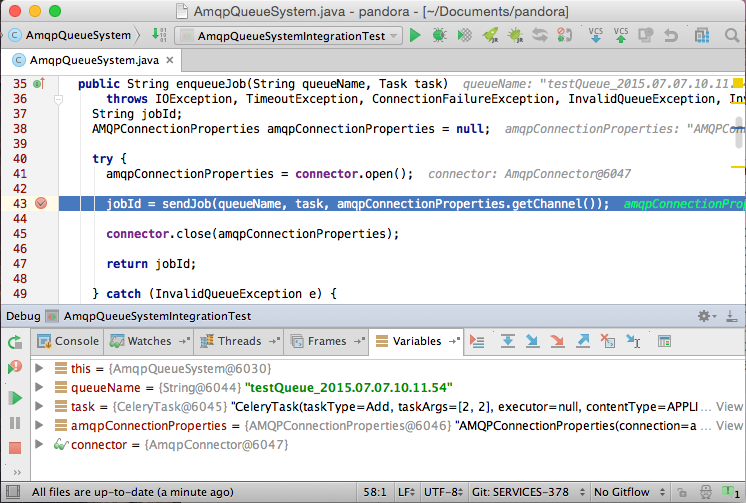
\includegraphics[scale=0.5]{intellijdebugger.png}
\chapter{How do I test my code?}
When you are developing your code, you can always manually test your code. However, manual tests are the worst kind of tests because there is no log of those tests and they are difficult to reproduce. Therefore, the team creates thorough unit and end-to-end tests for all new code.
\section{What are unit tests?}
A unit test is a test written by the programmer to verify that a relatively small piece of code is doing what it is intended to do. It should have \textbf{no dependencies} on code outside of the section being tested. They are narrow in scope, they should be easy to write and execute, and their effectiveness depends on what the programmer considers to be useful. The tests are intended for the use of the programmer, they are not directly useful to anybody else, though, if they do their job, testers and users downstream should benefit from seeing fewer bugs.\par
Part of being a unit test is the implication that things outside the code under test are mocked or stubbed out. Unit tests shouldn't have dependencies on outside systems. They test internal consistency as opposed to proving that they play nicely with some outside system.
\section{What are end-to-end / integration tests?}
An end-to-end / integration test is done to demonstrate that different pieces of the system work together. Integration tests cover whole applications, and they require much more effort to put together. They usually require resources like database instances and hardware to be allocated for them. The integration tests do a more convincing job of demonstrating the system works (especially to non-programmers) than a set of unit tests can, at least to the extent the integration test environment resembles production.\par
These tests are referred to as end2end tests in the Helios repo and integration tests in the Pandora repo, but they are the same thing.
\section{What is cobertura?}
Cobertura is a free Java tool that calculates the percentage of code accessed by tests. It can be used to identify which parts of your Java program are lacking test coverage. You can run cobertura through gradle, by clicking on the command shown below.\par
\begin{figure}[h!]
\centering
	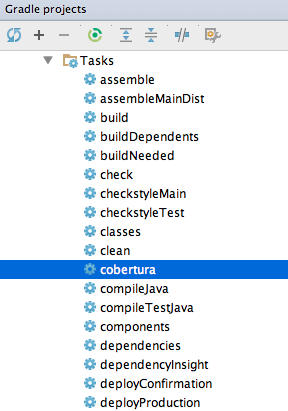
\includegraphics[scale=0.4]{cobertura.png}
\end{figure}
After running this command, you can access the report generated in a reports/cobertura folder. An example report is provided below:
\begin{figure}[h!]
\centering
	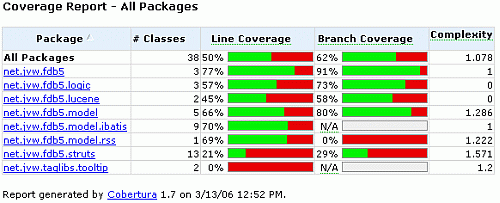
\includegraphics[scale=0.6]{coberturareport.png}
\end{figure}
\subsection{What is line coverage?}
Line coverage measures how many statements you took (a statement is usually a line of code, not including comments, conditionals, etc). The line coverage report represents \textbf{the percent of lines executed by the test run}.
\subsection{What is branch coverage?}
Branch coverages checks if you took the true and false branch for each conditional (if, while, for). You'll have twice as many branches as conditionals. The branch coverage report represents \textbf{the percent of branches executed by the test run}.
\subsection{Why should I care about the difference between line coverage and branch coverage?}
Consider the following example: \\
\begin{lstlisting}
public int getNameLength(boolean isCoolWikiaIntern) {
    User user = null;
    if (isCoolWikiaIntern) {
        user = new Connie(); 
    }
    return user.getName().length(); 
}
\end{lstlisting}
If you call this method with \texttt{isCoolWikiaIntern} set to true, you get 100\% line coverage. That sounds great, until you realize that there will be a \texttt{NullPointerException} if you call with \texttt{isCoolUser} set to false. However, you have 50\% branch coverage in the first case, so you can see there is something missing in your testing (and often, in your code).
\section{What are health checks?}
Every service has a health check. These tests are run periodically on the running application. They are meant to confirm that the service is able to successfully connect to any databases, servers, or other systems that it is dependent on. Health checks should connectivity, not functionality. Therefore, health checks should be fairly straightforward to create.
\section{Mocking}
Mocking is primarily used in unit testing. An object under test may have dependencies on other (complex) objects. To isolate the behavior of the object you want to test you replace the other objects by mocks that simulate the behavior of the real objects. This is useful if the the real objects are impractical to incorporate into the unit test.\par
n short, mocking is creating objects that simulate the behavior of real objects.
\subsection{Mockito}
Mockito is an open source testing framework for Java. Mockito allows the creation of mock objects in our unit tests. Below is an example of a unit test that uses Mockito.\\
\newline
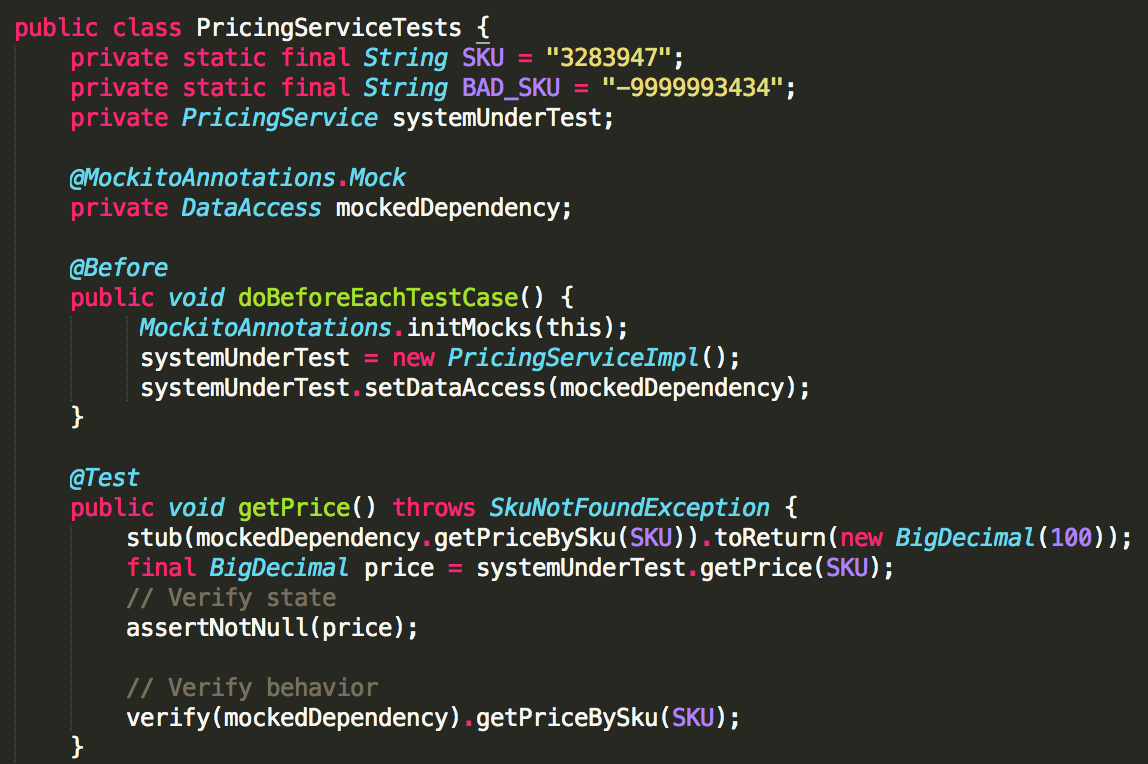
\includegraphics[scale=0.55]{mockito.png}
\chapter{Scrum Continued; How do I contribute to meetings?}
Whenever you are the newest joining member of a group, the rest of the members will have accumulated knowledge about the project that you are not privy to. Add being an intern fresh out of college on top of that, and team meetings can seem pretty intimidating.\par
Instead of dwelling on these fears, let's talk about how to mitigate them. This chapter will specifically focus on Scrum-style meetings, but the sentiments can be applied to joining any pre-existing team.
\section{Everyone knows so much! What ever will I do!}
No one in the meeting knows everything about all the moving parts. Usually, the team members have specialized knowledge on different aspects of the project. Use that to your advantage! If you don't know something, \textbf{ask}. Odds are you aren't the only one who doesn't know all the ins and outs of the current task.\par
Additionally, explaining a project component in detail can be helpful to the developer as well. Being able to clearly and concisely explain what you are doing and why you are doing it is a major component of development. 
\section{How do I gain a deeper understanding of the project?}
\subsection{Backlog Grooming}
During backlog grooming, the team comes together to look over the tickets in the backlog. They add new stories and epics, extract stories from existing epics, and estimate effort for existing stories. Basically, this is your chance to get up to date on everything you missed before you joined the team! Pay close attention during these meetings to understand what every story consists of and ask questions about anything you don't understand.
\subsection{Sprint Planning}
Every iteration begins with the sprint planning meeting. At this meeting, the Product Owner and the team negotiate which stories a team will tackle that sprint. During this meeting, you have a chance to fully understand all of the stories that the team will be working on this sprint and be up to date with what everyone on the team is doing. \par
When you estimate the amount of effort to assign each story, you will gain a better understanding of all that moving parts that the story involves. 

Take advantage of this meeting! It will help you stay up-to-date on all the upcoming stories and contribute meaningfully in future meetings.
\chapter{Payroll? Hours? What is going on!}
Interns are on payroll, so we need to log our hours every two weeks. Wikia uses ADP, \texttt{https://workforcenow.adp.com}. HR can provide you with the details on registration. Once you are registered, you will be able to log into ADP and enter your hours. Once they are entered, make sure it approve your timesheet and have your manager approve it as well.
\chapter{Writing your first API; Rambling Advice}
When writing an interface, think about what the client needs to know. \textbf{Only} include what the client needs to use/know about that service. Everything else is implementation, and should be abstracted away. \par
When writing services, make your service as general as possible. I ran into this issue often where I would accidentally make my service too specific to our current implementation without even realizing.\par
When naming, think about making your names as specific and clear as possible. Unclear names make for frustrating code. \par
Whenever you write/do anything, be \textbf{intentional}:
\begin{itemize}
	\item What package you put your file in
	\item The name of that package
	\item The name of your class
	\item The way work is divided among methods
\end{itemize}		
It’s not just about getting the job done and working ; it’s about making code that easy to understand and change when necessary
\chapter{Mistakes I've made}
I have a ton more to add to this list, these are just a few things that come to mind:
\begin{itemize}
	\item On Git, I deleted a file without knowing it. (Ended up spending half and hour debugging the issue before going to Nelson.) What did I learn? Always \texttt{git status} before committing!
	\item For my first API, I wrote interfaces that were so specific they didn't serve a purpose. That experience inspired the last chapter. What did I learn? Keep everything generic! Make sure the API does not reference your implementation.
	\item Sometimes, I had pretty off days. I would put in my best effort, but I'd still end up making silly mistakes or misunderstanding simple concepts. What did I learn? Not everyday will be your best day, so don't be too hard on yourself.
	\item This isn't a mistake, but best of luck! You're going to do great :-)
\end{itemize}
\end{document}